\documentclass[utf8x]{beamer}
\usepackage[czech]{babel}

\usetheme{Madrid}
\setbeamertemplate{footline}[frame number]

\title{Konečné automaty}
\author{Dominik Večeřa}
\date{28. 4. 2018}
\institute[Brno University of Technology]

\begin{document}

\begin{frame}
  \titlepage
\end{frame}

\begin{frame}{Obsah}
  \tableofcontents
\end{frame}

\section{Definice}

\subsection{Definice}

\begin{frame}{Konečný automat}
  \begin{itemize}[<+->]
  \item {
    \textbf{Konečný automat} je teoretický výpočetní model používaný v informatice pro studium formálních jazyků.
  }
  \item {
    Popisuje velice jednoduchý počítač, který se může nacházet v jednom z několika stavů, mezi nimiž přechází na základě symbolů, jež čte ze vstupu.
  }
  \item{
    Množina stavů je konečná (odtud název), automat nemá žádnou další paměť kromě informace o svém aktuálním stavu.
  }
  \end{itemize}
\end{frame}

\subsection{Formální definice}

\begin{frame}{Formální definice}

  Formálně je konečný automat definován jako uspořádaná pětice ($S,\Sigma,\sigma,s,A$), kde:
  \pause
    
  \begin{itemize}[<+->]
  \item {   
    S je konečná neprázdná množina stavů.
  }
  \item {   
    $\Sigma$ je konečná neprázdná množina vstupních symbolů, nazývaná \textit{abeceda}.
  }
  \item {   
    $\sigma$ je tzv. \textit{přechodová funkce} (též \textit{přechodová tabulka}), popisující pravidla přechodů mezi stavy. Může mít buď podobu $S \times \Sigma \rightarrow S$ (deterministický automat), nebo $S \times \{\Sigma \cup \epsilon\} \rightarrow P(S)$ (nedeterministický automat).
  }
  \item {   
    \textit{s} je \textit{počáteční stav}, $s \in S$.
  }
  \item {   
    \textit{A} je množina \textit{přijímajících stavů}, $A \subseteq S$.
  }
  \end{itemize}
\end{frame}

\section{Činnost automatu}

\subsection{Popis činnosti automatu}

\begin{frame}{Popis činnosti automatu}

Nejprve se automat nachází v definovaném počátečním stavu. S každým dalším krokem poté přečte jeden symbol ze vstupu a přejde do stavu daného hodnotou v přechodové tabulce odpovídající aktuálnímu stavu a symbolu, jež byl přečten.

\pause
\vspace{3mm}

Podle toho, zda automat skončí po přečtení vstupu ve stavu, který patří do množiny přijímajících stavů, platí, že automat buď daný vstup přijal, nebo nepřijal. Množina všech řetězců, které daný automat přijme, tvoří regulární jazyk.
    
\end{frame}

\subsection{Příklad jednoduchého automatu}

\begin{frame}{Příklad jednoduchého automatu}

\begin{center}
    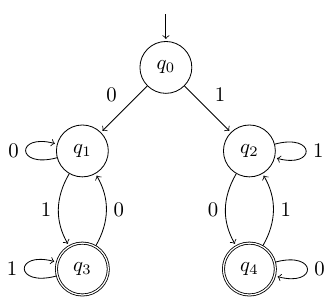
\includegraphics[]{konecny-automat.png}
\end{center}

Postup automatu je určen posloupností jedniček a nul na vstupu.

\end{frame}

\begin{frame}{Deterministický vs. nedeterministický automat}
    \begin{block}{Deterministický konečný automat}
        je charakteristický tím, že se vždy nachází právě v jednom ze svých vnitřních stavů.
    \end{block}
    
    \begin{block}{Nedeterministický konečný automat}
        je charakteristický tím, že se může v jednom okamžiku nacházet v celé množině svých vnitřních stavů (tedy více než v jednom). Nedeterministické konečné automaty lze převést na deterministické, čímž se však zvýší počet stavů.
    \end{block}
\end{frame}

\appendix

\begin{frame}{Použité zdroje}
\begin{thebibliography}{}

\bibitem{} Matematika.cz:
    \emph{Konečný automat}. [online], [citováno 28. 4. 2018].\\
    Dostupné z: \texttt{https://matematika.cz/konecny-automat}
\vspace{2mm}
\bibitem{} Wikipedia.org:
    \emph{Konečný automat}. [online], [citováno 28. 4. 2018].\\
    Dostupné z: \texttt{https://cs.wikipedia.org/wiki/Konečný\_automat}
\vspace{2mm}
\bibitem{} HORDĚJČUK, V.:
    \emph{Konečný automat}. [online], [citováno 28. 4. 2018].\\
    Dostupné z: \texttt{http://voho.eu/wiki/konecny-automat/}

\end{thebibliography}
\end{frame}
\end{document}